%=====================
\chapter{Introduction}
%=====================

This chapter is a technical introduction to our project.
It gives a concise explanation of the most important terms used in the report.

The first section briefly explains \Gls{wireshark}, \glspl{dissector} and how \glspl{dissector} are used in \Gls{wireshark}.
The connection between \Gls{wireshark} and the \Gls{lua} \glspl{struct} \gls{protocol} is also explained.

The second section describes how the \Gls{lua} code works and how it is generated by our \gls{utility}.

%---------------------------------
\section{Wireshark and Dissectors}
%---------------------------------
This section gives a brief introduction to \Gls{wireshark} and \glspl{dissector}.
The first part describes what \Gls{wireshark} is and what it can be used for.
The second part explains exactly what a \gls{dissector} is, and how a \gls{dissector} can be used to extend \Gls{wireshark}.

\subsection{Wireshark}
%---------------------
\Gls{wireshark} is a program used to analyze network traffic. A common usage scenario is when a person wants to troubleshoot network problems or
look at the internal workings of a network \gls{protocol}. An important feature of \Gls{wireshark} is the ability to capture and display a live stream of \glspl{packet} sent through the network. 
A user could, for example, see exactly what happens when he opens up a website. \Gls{wireshark} will then display all the messages
sent between his computer and the web server. It is also possible to filter and search on given \gls{packet} attributes, which facilitates the debugging \gls{process}.

In \autoref{fig:introshark}, you can see a view of \Gls{wireshark}.
This specific example shows a capture file with four messages, or \glspl{packet}, sent between internal \glspl{process}, in other words
it is a view of messages sent by inter-\gls{process} communication. Each of the \glspl{packet} contain one \Gls{c} \gls{struct}.
To be able to display the contents of the \Gls{c} \gls{struct}, \Gls{wireshark} must be extended. 
This can be accomplished by writing a \gls{dissector} for the \Gls{c} \gls{struct}.

\Gls{wireshark} \glspl{dissector} can be written in either \Gls{c} or \Gls{lua}, and in our \gls{utility} they are written in \Gls{lua}.
The difference between \Gls{c} and \Gls{lua} \glspl{dissector},
and the reason we used \Gls{lua} is elaborated on in the 
preliminary study in \autoref{cha:prestudy}.
Dissectors, in general, are explained more in detail below.

\begin{figure}[htb]
	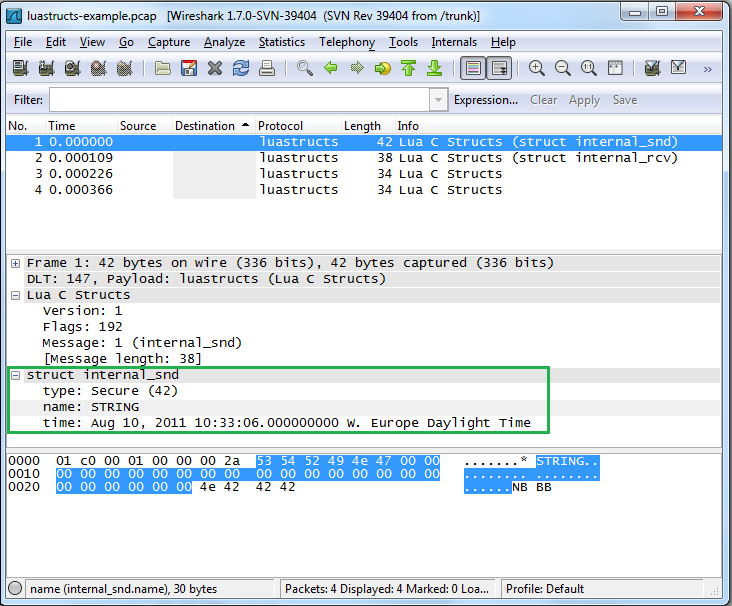
\includegraphics[width=\textwidth]{./planning/img/wireshark_example}
	\caption{Wireshark Screenshot\label{fig:introshark}}
\end{figure}

\subsection{Dissectors}
%----------------------
In short, a \gls{dissector} is a piece of code run on a blob of data, which can dissect the
data and display it in a readable format in \Gls{wireshark}, instead of the \gls{binary} representation.

\autoref{fig:introshark} displays four \glspl{packet}, with \gls{packet} number 1 highlighted.
The content of the \gls{packet} is a \Gls{c} \gls{struct} with three \glspl{member}, type, name and time, and is displayed inside the box in the figure.
The \Gls{c} code for the \gls{struct} is shown in \autoref{structexample}.
The \gls{dissector} takes the \Gls{c} \gls{struct}, decodes its \gls{binary} representation and makes it readable by humans.
Without a \gls{dissector}, \Gls{wireshark} would just display the \gls{struct} and \gls{struct} \glspl{member} as a \gls{binary} blob.

All the \glspl{packet} containing \Gls{c} \glspl{struct} belong to the \gls{protocol} called luastructs.
When opening a capture file in \Gls{wireshark} , this \gls{protocol} maps the id of the messages to the correct \gls{dissector},
and calls them.

\lstset{language=C,caption={Example C Struct},label=structexample}
\lstinputlisting[language=C]{./planning/code/struct.h}

%------------------------------------------------------------------
\section{From \Gls{struct} Definition to \Gls{lua} \Gls{dissector}}
%------------------------------------------------------------------
This section explains what happens under the hood of a \Gls{lua} \gls{dissector}.

\begin{comment}
, and how they can be built by our \gls{utility}.
The first part explains what happens under the hood of a \Gls{lua} \gls{dissector}, while 
the second part is a very brief explanation of how CSjark builds such \glspl{dissector}.
\end{comment}

\subsection{\Gls{lua} \Glspl{dissector}}
%---------------------------------------
\autoref{luaexample1} shows what the code for the \Gls{lua} \gls{dissector}, used to display the content of \gls{packet} 1 in \autoref{fig:introshark}, looks like.
The Proto variable defines a new \gls{protocol}. In this example, a \gls{dissector} for the internal\_snd \gls{struct}, called internal\_snd, is created. 
The different fields of the \gls{struct} are created as instances of ProtoField, and put into Protocol.fields.
For example, the ''name'' variable is a \gls{string} in \Gls{c}, and as such it is created as a ProtoField.\gls{string} with the 
name ''name''.

The \gls{protocol} \gls{dissector} function is the function that does the actual dissecting.
A subtree for the \gls{dissector} is created, and the description of the \gls{dissector} is appended to the information column.
All the ProtoFields are added to the subtree. Here you can see that the type, name and time fields are added for the internal\_snd \gls{dissector}.
The content of the subtree is what is actually displayed when a \gls{struct} is dissected in \Gls{wireshark}.
The buffer size allocated to the fields is the size of the \glspl{member} in \Gls{c}.

In the last line the \gls{dissector} is added to the \gls{dissector} table as a subdissector for the luastructs \gls{protocol}.
When running a capture file, where the internal\_snd \gls{struct} is being sent to another \gls{process}, it is possible to see the exact contents of the \gls{struct}. An example of this is shown in \autoref{fig:introshark}.

\newpage
\lstset{language=C,caption={Example Lua File},label=luaexample1}
\lstinputlisting[language=C]{./planning/code/luaexample1.lua}

\begin{comment}
\subsection{CSjark - Automated generation of \Gls{lua} \glspl{dissector}}
CSjark is a \Gls{python} \gls{utility} that can automatically generate a \Gls{lua} \gls{dissector} for 
any valid \Gls{c} \gls{header} file. It also supports user configuration from files in a specific format.
The \Gls{c} file, in addition to any suitable configuration file, is inputted into a command line interface.
The \Gls{c} file is then sent to the \Gls{c} preprocessor, where \Gls{c} directives are evaluated before the parsing.
The \gls{parser} creates an abstract syntax tree from the input.
CSjark traverses the abstract syntax tree and finds all the \gls{struct} definitions.
For every \gls{struct} that is found, a \gls{dissector} is generated and written to file.
\end{comment}

